\section{METHOD}
\label{sec:method}

For tackling the here proposed problem, a YOLO detector has been used at first. The YOLO network usually relies on Darknet, an open source neural network framework written in C and CUDA. However, we initially relied on a popular python translation of Darknet, called Darkflow, to set up the learning pipeline. Since Darkflow does not support YOLO v3 yet, we used YOLO v2 as the model to be fine-tuned for an initial testing. Anyway, this approach did not yield any good result, with the network not being able to properly converge. A variety of setups of parameters were tried, but the loss and moving average loss values never decreased under the approximate threshold of 30 (starting from about 130). In particular, the learning rate has ranged from $1 \cdot 10-3$ to $5 \cdot 10-7$ with a step of a 10 factor and fixed decay equal to $5 \cdot 10-4$, batch size has ranged from 1 to 64 with step 8, and both ‘Adam’ and ‘sgd’ optimizers have been tested. Moving to YOLO v3 using an open source Keras implementation resulted approximately in the same bad performance with the same setups. The training was performed both using and not using different weights pretrained on COCO dataset, namely those provided by Joseph Redmon via the official website of the YOLO project. In light of these results, a different approach has been preferred. Instead of using an end-to-end model to detect bounding boxes and translate each character, we pipelined two different models: 1) a model to detect the characters and 2) a model to predict the specific Japanese character from each detected object. In particular, we implemented a CenterNet architecture for detection and a quite simple CNN for classification. The name CenterNet is used because the architecture is taken by the paper “Objects as Points” which uses this same name.

\subsection{Character detection using CenterNet}
\label{ssec:charactercenternet}

In the referenced paper, the authors propose a deep neural network for object detection and classification tasks called CenterNet. The difference with other object detection networks is that CenterNet predicts the position of a variable number of keypoints in the image, leaving the task of inferring bounding boxes to a post-processing operation. The aim of this network is hereby described reporting some information and notations from the official paper. Let $I \in R^{W \times H \times 3}$ be an image of height $H$, width $W$ and 3 channels. CenterNet will predict a heatmap  $Y \in [0,1]^{\frac{W}{R} \times \frac{H}{R} \times C}$, where $R$ is the output stride of the network and $C$ is the number of keypoint types, which is the number of categories to be predicted. $R$, the output stride, is the scale factor of the network (in our case, since we worked with squared images, measured as input widthoutput width). With respect to the predicted heatmap:
\begin{itemize}
	\item A prediction $\hat{Y}_{x,y,c}=1$ means that a keypoint of type $c \in C$ has been detected in position $(x \cdot R, y \cdot R)$ of the input image.
	\item A prediction $\hat{Y}_{x,y,c}=0$, corresponds to a background point (i.e. non-keypoint).
\end{itemize}

\subsubsection{Implementation}
\label{sssec:implementationdet}

To implement the detection model we followed both the implementation described in the paper and an existing implementation created by a Kaggle user specifically for the purpose of the competition\footnote{Available here: \url{https://www.kaggle.com/kmat2019/centernet-keypoint-detector}}.\\ We call this model the \textit{detector model}, since its purpose is detecting the center of each character to be recognised in the image. Note that in our implementation there is just one type of keypoint that should be recognised. However, as reported in the paper, CenterNet allows to use more keypoint types (e.g. it has been used in human pose recognition task, where each keypoint type represented a different human joint). Theoretically it may be possible to use this same architecture also for character classification, using a different keypoint type for each Kuzushiji character. However, the number of classes (in subset $C$) would be very high (i.e. $>$ 4200) and consequently the output of the model would be huge and impractical to manipulate, additionally resulting in a higher training and predict time. Thus, we preferred the two steps approach, using different models for detection and classification.

\subsubsubsection{Description of the input samples}
\label{ssssec:inputsamples}

Firstly, each training image is randomly cropped and resized to the input dimension, which was set to $512 \times 512$. Then, the output of the training sample is generated using the annotations created during the preprocessing step. For each keypoint $p$, a downsampled point is computed as $\hat{p}=\left\lfloor \dfrac{p}{R} \right\rfloor$, which represents the point in the output space.\\
The heatmap is generated with a gaussian function applied to each pixel of the image as in equation \ref{eq:gaussian}.
\begin{equation}\label{eq:gaussian}
	Y_{x,y,c}=\exp\left(\dfrac{1}{2} \cdot \left(\frac{x-p_x}{\sigma}\right)^2 \cdot \left(\frac{y-p_y}{\gamma}\right)^2 \right)
\end{equation}
In the equation we set $\sigma = \dfrac{w}{10}$ and $\gamma = \dfrac{h}{10}$, where $w$ and $h$ are the image width and height respectively.\\
For the purpose of our project, the heatmap slightly differs from the one described in the original paper. The implementation we opted for has been used in the aforementioned Kaggle notebook, and allows the creation of heatmaps such that the keypoint heat can form elliptic shapes and not only perfect circles. In addition, to recover from the discretization error caused by the output stride, we also add a local pixel offset $\hat{O} \in R^{\frac{W}{R} \times \frac{H}{R} \times 2}$(as in \cite{CenterNet2019}). For example, if a keypoint location in the image is $(12.32, 122.18)$ the offset will be of $(0.32, 0.18)$ with the values divided by the output stride.
Finally to predict the bounding box for each object we add information about the object size $\hat{S} \in R^{\frac{W}{R} \times \frac{H}{R} \times 2}$. This size is computed as $(xmax-xmin, ymax-ymin)$, divided by the output size, which in our case is 128. Each training example is then fed to the network. Summing up, the shape of each input image is (512, 512, 3), while the target output $Y_{x,y,c}$ for each example has shape (128, 128, 6), where:

\begin{itemize}
	\item $Y_{x,y,0}$ contains the gaussian heatmap;
	\item $Y_{x,y,2}$ is the width offset;
	\item $Y_{x,y,3}$ is the height offset;
	\item $Y_{x,y,4}$ and $Y_{x,y,5}$ are respectively the width and height estimation for the bounding box.
\end{itemize}

We followed the implementation on Kaggle adding in $Y_{x,y,1}$ the “ground truth map” with 1 in correspondence of centers and 0 for all other points. This map is used to compute the loss function as described in the next paragraph.

\subsubsubsection{Loss function}
\label{ssssec:lossfunctiondet}

We used the loss functions provided in the Kaggle implementation, which follow the description of the paper. The main loss function is computed from three separate losses $L_h$, $L_o$, $L_s$, that measure the error on the heatmap, offset and size respectively. The heatmap loss is defined as (\ref{eq:heatloss}):
\begin{equation}\label{eq:heatloss}
L_h=-\dfrac{1}{N}\sum_{x,y}
\begin{cases}
(1-\widehat{Y}_{x,y,0})^{\alpha} \\~~~~\cdot \log(\widehat{Y}_{x,y,0} + \epsilon)~~~~~~~~~~\text{if}~Y_{x,y,0} = 1 \vspace*{10pt} \\
(1-Y_{x,y,0})^{\beta} \cdot (\widehat{Y}_{x,y,0})^\alpha \\ ~~~~\cdot \log(1-\widehat{Y}_{x,y,0} + \epsilon) ~~~~~~\text{if}~Y_{x,y,0}=0
\end{cases}
\end{equation}
where $\alpha=2$ and $\beta=4$ as suggested in the paper, while $\epsilon=1 \cdot 10-6$ is a small constant added to the log argument to avoid getting it to 0. Note that in the original paper the sum was done over all $x$, $y$, $c$, but in our implementation we want to predict one keypoint type only, so in the formula we substituted the c variable with 0.
The other losses are defined as:
\begin{equation}
L_o = \dfrac{1}{N}\sum_{k=1}^{2}\sum_{x,y}\left|Y_{x,y,k+1} - \widehat{Y}_{x,y,k}\right|
\end{equation}
\begin{equation}
	L_s = \dfrac{1}{N}\sum_{k=3}^{4}\sum_{x,y}\left|Y_{x,y,k+1} - \widehat{Y}_{x,y,k}\right|
\end{equation}

\noindent Hence, the final loss is obtained as:
\begin{equation}
	L=L_h+ \lambda_1 \cdot L_o+ \lambda_2 \cdot L_s
\end{equation}
with $\lambda_1=1$ and $\lambda_2=5$, the same values used in the paper.

\subsubsubsection{Network architecture}
\label{ssssec:networkarchitecturedet}

The network follows the encoder-decoder architecture similar to the one used in U-Net. As an encoder we used both ResNet34 and ResNet50, removing the last average pooling and fully connected layers. On top of the encoder we added the decoder, as a stack of three up-convolutional layers. This architecture is the simplest among those described in the CenterNet research paper. In addition, following the U-Net architecture we added some cross connections from the encoder to the decoder.\\
Note that in the following description we will not specify the 2D or 3D nature of image transformations (like convolution), since all the operations we performed are bidimensional.\\
The full architecture diagram using ResNet34 is shown in figure \ref{fig:detector}. For ResNet50 we used the pre-trained model available in Keras, initialized with the weights used for ImageNet.\\

\begin{figure}[h]
	\caption{Architecture of the detector model.}
	\centering
	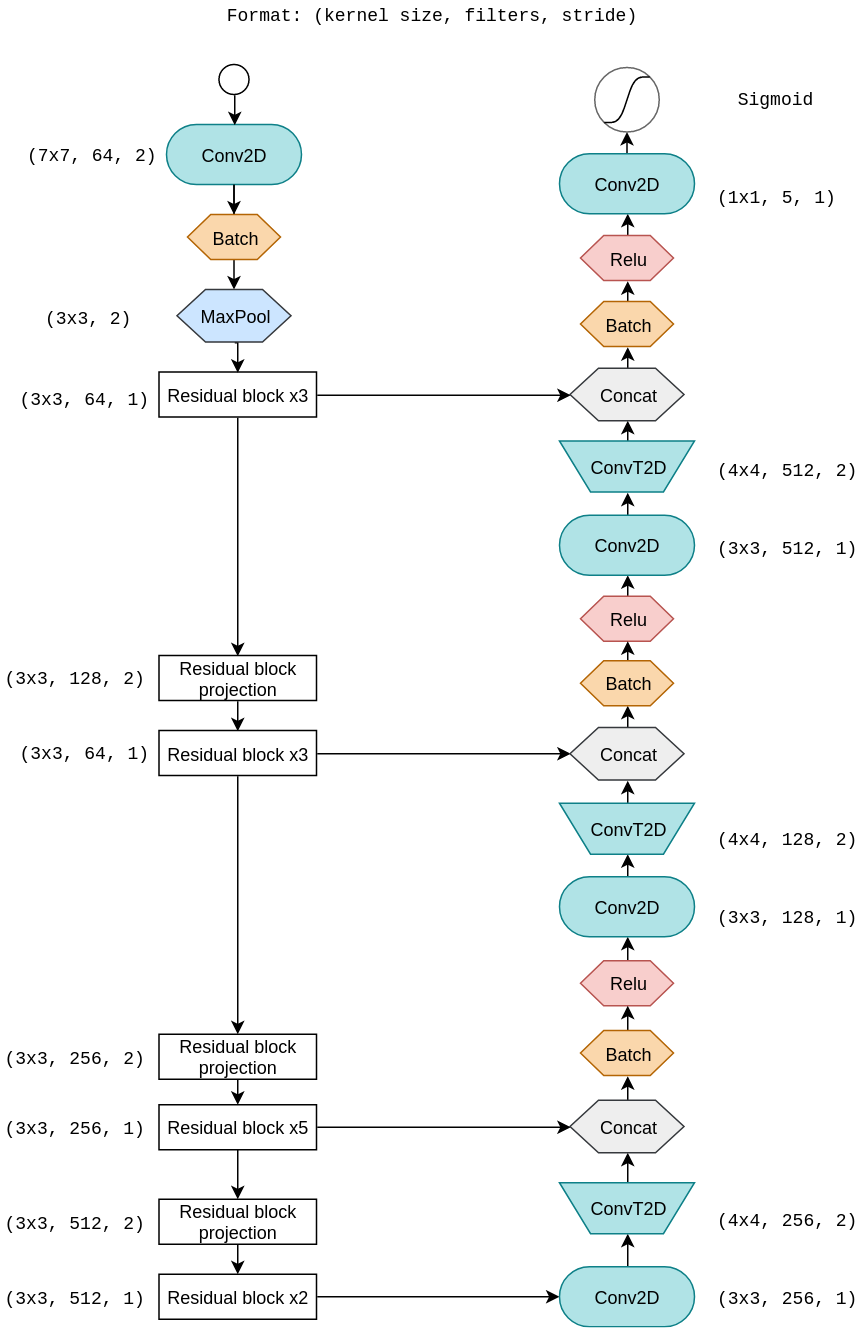
\includegraphics[width=0.45\textwidth]{architectures/detector.png}
	\label{fig:detector}
\end{figure}

\noindent During the encoding phase, the input image of dimension $512 \times 512$ is shrunk through 5 convolutional blocks.\\
The first block uses a convolution of size 7 and stride 2 and a max pooling operation to downsample the image by a factor of 4.\\
The second block is built of 3 standard residual blocks with identity shortcut. Such a block can be visualized in figure \ref{fig:resblock_1}. These blocks do not change the image dimension and they just apply two convolutions to add more feature maps, with the additional layer at the end.\\
The third block halves the image size using a residual block with projection shortcut (in figure \ref{fig:resblock_2}) and three residual blocks with identity shortcut.\\
Fourth and fifth blocks just repeat this steps with a different number of identity shortcut blocks. Note that each residual block double the number of channels in the image. For what concerns the decoder, the encoded input of size $(16, 16, 512)$ is passed to the decoder that uses three up-convolutional blocks to upsample it to the desired output dimension of $(128, 128, 5)$. Here, we made two major changes with respect to the standard CenterNet implementation of the decoder:

\begin{enumerate}
	\item We added cross connections in U-Net fashion, and
	\item We replaced the deformable convolution layer with a simple convolution.
\end{enumerate}

\begin{figure}[h]
	\caption{Residual block with identity shortcut.}
	\centering
	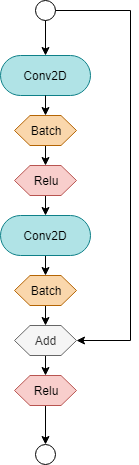
\includegraphics[width=0.1\textwidth]{architectures/resblock_1.png}
	\label{fig:resblock_1}
\end{figure}

\begin{figure}[h]
	\caption{Residual block with projection shortcut.}
	\centering
	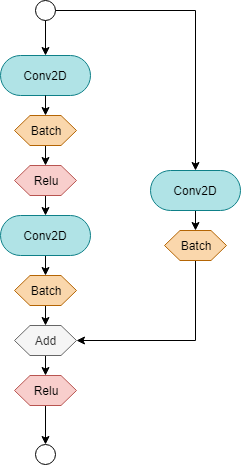
\includegraphics[width=0.2\textwidth]{architectures/resblock_2.png}
	\label{fig:resblock_2}
\end{figure}

The difference between a standard convolution and deformable convolution is that using the former the receptive field and the sampling locations are fixed all over the top feature map, while using the latter they are adaptively adjusted according to the scale and shape of the objects in deformable convolution. This is implemented by augmenting the standard convolutional grid with a matrix of parameters called offsets, which must be learned in addition to the standard convolution weights \cite{DeformableConv2017}. The authors of the original paper reported an improvement over standard convolution for object detection tasks, in particular in the detection of irregular objects. On the other hand, the characters to be recognised in the Kuzushiji documents are arranged in adjacent columns, in a grid-like pattern. For this reason, and considering the additional computational time required to train a deformable convolutional network, we decided to replace them with their standard counterparts. \\

The decoder is composed of three identical blocks, each featuring the following layers:

\begin{itemize}
	\item a convolution to reduce the number of features;
	\item a transposed convolution to upsample the image by a factor of 2;
	\item a concatenate operation that concatenates the output of a block of the encoder with the output of the transposed convolution;
	\item a batch normalization to reduce variances of values;
	\item a leaky ReLu activation.
\end{itemize}

The last block is composed of a $1 \times 1$ convolution to reduce the number of features to 5 and a sigmoid activation. The final output is an array with 3 dimensions shaped as $(128, 128, 5)$. This output is the predicted heatmap $\widehat{Y}$. Each of the five layers in the outer dimension has the same meaning explained above, with the difference that the “ground truth map” is not predicted, since this information is provided inside the heatmap itself. This is the reason why the output has 5 instead of 6 layers for each image.

\subsubsection{Pre-processing and training}
\label{sssec:preprocessingdet}

The input samples are firstly resized to $512 \times 512 \times 3$ and normalized, as well as random cropped for data augmentation. A maximum crop factor is determined considering the average character size in the page. This is determined separatedly for width and height as shown in equations \ref{eq:stretchw} and \ref{eq:stretchh}, where $w$ and $h$ are the dimensions of the original image and $char\_area$ is the average bounding box area within the page.
\begin{equation}\label{eq:stretchw}
	c_w=\sqrt{\frac{w \cdot h}{char\_area}}
\end{equation}
\begin{equation}
\label{eq:stretchh}
	c_h=\frac{h}{w}\sqrt{\frac{w \cdot h}{char\_area}}
\end{equation}
This crop procedure allows to train the network on smaller fragment of pages with better recognition rate of small sharacters. In addition, this step ensures good recognition performances when paired with the post-processing passage described in the next section.\\
\noindent Finally, all output classes, expressed as unicode characters, are mapped to integer values.

\subsubsection{Post-processing: from centers to bounding boxes}
\label{sssec:preprocessingandtraining}

The previously described network predicts the location of the center of each character within the page. From that we infer the coordinates of the bounding box location using the size information in the predicted heatmap ($Y_{x,y,3}$ and $Y_{x,y,4}$) and summing the offsets ($Y_{x,y,1}$ and $Y_{x,y,2}$). To further improve the accuracy of the bounding boxes, some post-processing has been made as well. Firstly, all heatmap elements with score prediction below 0.7 were filtered out, since they probably represent noise. The remaining ones are the predicted centers. The predicted offsets are then added to the coordinates of these centers in the heatmap and the definitive coordinates of the bounding boxes are computed as:
\begin{eqnarray*}
	xmin=x_c - \frac{width}{2}\\
	ymin= y_c - \frac{height}{2}\\
	xmax=x_c + \frac{width}{2}\\
	ymax=y_c + \frac{height}{2}
\end{eqnarray*}
Then, out-of-picture boxes and the ones with an area too different from the average area in the page (too big or too small) are removed. Finally overlap-based non maximum suppression is performed comparing the intersection area between the boxes. Each lower score bounding box sharing more than 40\% of the area of higher score boxes, or having more than 60\% of its area inside other higher score bounding boxes is removed.\\

\noindent Despite the non-maximum-suppression, we noted that some small characters were not detected by the network. This happens because the feature map is, in some cases, too small with respect to the original image, and may lose some information, leading to lower IoU score with the ground truth bounding boxes. 
Our solution was to divide each image into a number $n$ of smaller images (that we call \textit{tiles}) and use the model to predict bounding boxes in each one of the smaller images. A 25\% overlap between the tiles is used to preserve the objects along the tile boundaries and prevent any miss due to image partitioning. An example of partitioned image is shown in figure \ref{fig:tiles4}.

\begin{figure}
	\centering
	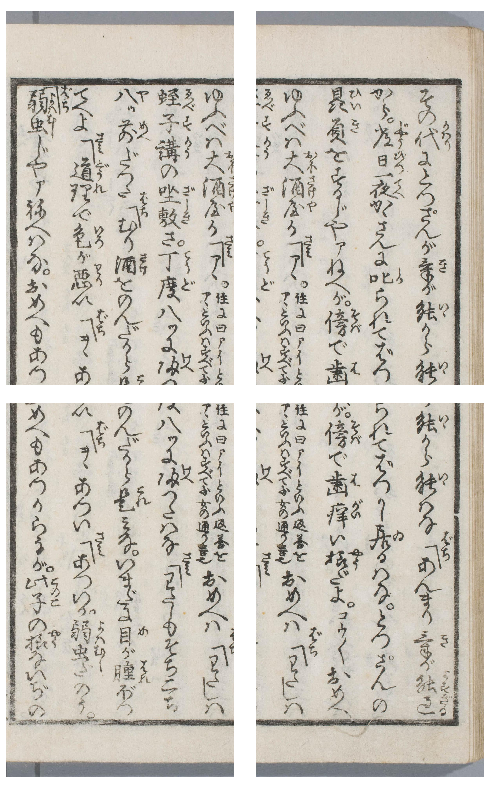
\includegraphics[width=0.8\columnwidth]{detection/tiles_4.png}
	\caption{An image divided in 4 tiles with 25\% overlapping}
	\label{fig:tiles4}
\end{figure}

This procedure resulted in more precise bounding box predictions and an higher IoU score on the test set. A comparison can be seen in figure \ref{fig:comparisontiling}. \\
We empirically determined the optimal number of tiles by measuring the IoU score over the same first 100 examples of the test set. Results gave a 0.7731 score using a $2 \times 2$ grid and 0.7850 using a $3 \times 3$ grid. 
Since the difference in the IoU score was negligible we chose to use a $2 \times 2$ grid, with the benefit of halving the time required to generate predictions for a single image.\\
It's worth to say that the same model trained without the random crop described in §\ref{sssec:preprocessingdet} did not reach such scores, but rather got an average IoU score of 0.53. This probably means that the crop procedure enhances the ability of the model to detect small features, particularly useful when predicting portions of images.

\begin{figure*}[h!]
	\centering
	\begin{subfigure}{\columnwidth}
		\centering
		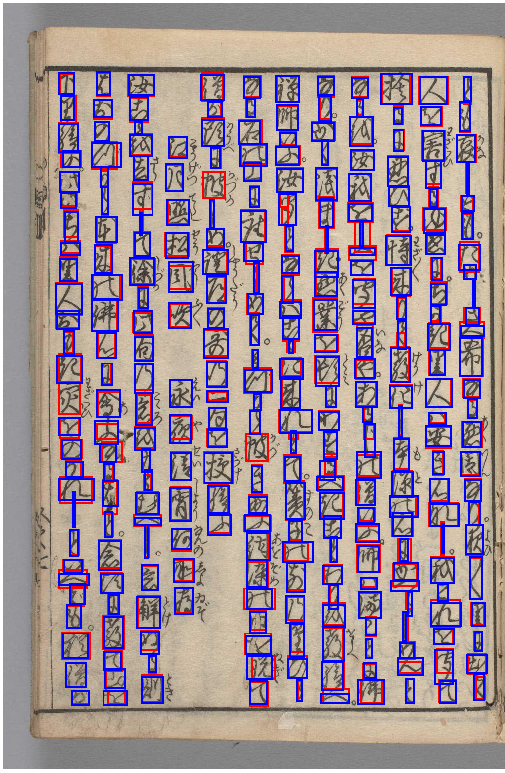
\includegraphics[width=0.9\columnwidth]{detection/tiled_prediction.png}
		\caption{Predicion with $2\times2$ tiling}
		\label{fig:tiledpred}
	\end{subfigure}
	\begin{subfigure}{\columnwidth}
		\centering
		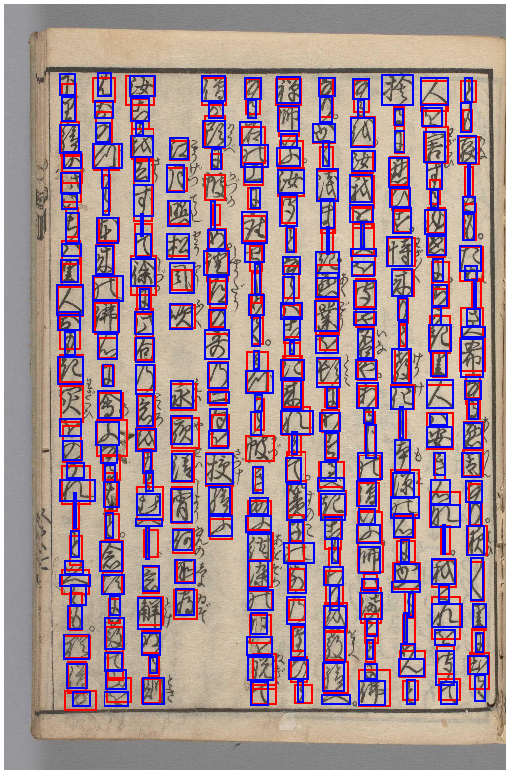
\includegraphics[width=0.91\columnwidth]{detection/standard_prediction.png}
		\caption{Predicion with no tiling}
		\label{fig:standardpred}
	\end{subfigure}
	\caption{Comparison of predicion on the same page with or without tiling. Image (\ref{fig:tiledpred}) has a IoU score of 0.83, while (\ref{fig:standardpred}) scored 0.59.}
	\label{fig:comparisontiling}
\end{figure*}

\subsection{Classification of characters using a standard CNN}
\label{ssec:classificationcnn}

While the model described in the previous section was used to detect characters, the goal of the classifier is to classify each detected character in one of the 4212 current Japanese characters, hopefully the one corresponding to its translation. The number of classes in our model is the number of different Kuzushiji characters found in the training set. In the official dataset for the competition, a dictionary of 4787 Kuzushiji characters and their translation was provided, but not all of them are present in the training set, while other characters are extremely rare. This may lead to worse classification performances for characters the model has seen fewer times.

\subsubsection{Implementation}
\label{sssec:implementationclass}

\subsubsubsection{Network architecture}
\label{ssssec:networkarchitectureclass}

The classifier is a small convolutional model based on the one proposed in the Kaggle implementation. The architecture diagram is shown in figure \ref{fig:classifier}. The three repeated blocks are followed by an average pooling layer with kernel size equal to the input dimension (named global pooling), which produce a single value for each feature map. This value is then fed to the final dense layer with softmax activation and number of units equal to the number of categories. We tested some simple variations using different types of residual blocks, and they worked equally well, so we didn not spend much time experimenting with other architectures.

\begin{figure}[h]
	\caption{Architecture of the classifier.}
	\centering
	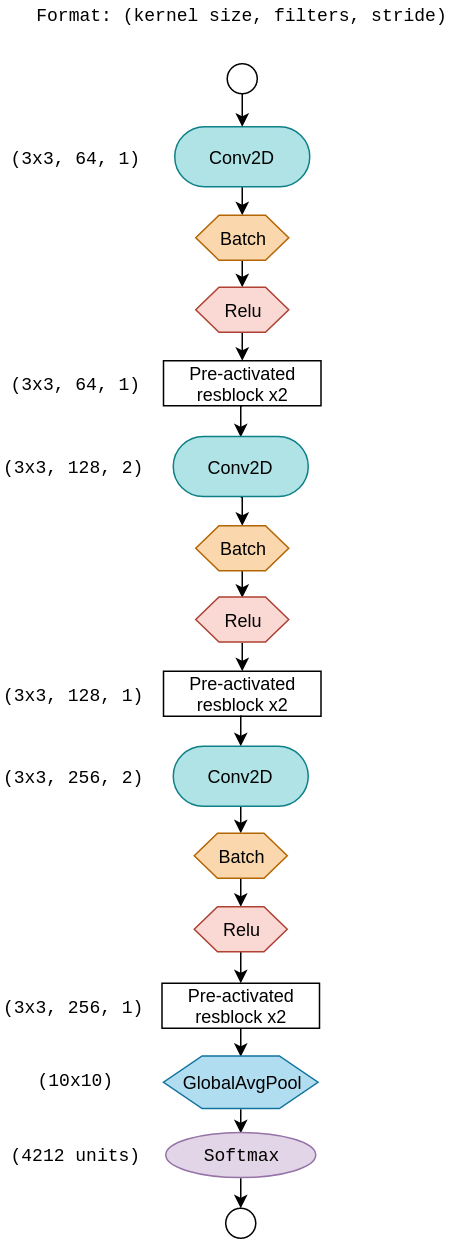
\includegraphics[width=0.25\textwidth]{architectures/classifier.png}
	\label{fig:classifier}
\end{figure}

\subsubsubsection{Loss function}
\label{ssssec:lossfunctionclass}

Since the character classes are codified as integers, we used sparse categorical crossentropy to evaluate the error of the model. 

\subsubsection{Pre-processing and training}
\label{sssec:preprocessingclass}

In order to deal with the main challenging features of cursive handwritten text, some data augmentation has been made on the $32 \times 32$ cropped and resized images of the detected characters. In particular, the objective was emulating the imprecision, variability and deformation inherent the writing of the characters. For this purpose, the dataset has been augmented with copies of the original images slightly altered with respect to brightness, rotation, width and height shifts, and zoom. The augmentation has been performed using the \textit{ImageDataGenerator} utility provided by Keras. 
We trained the classification network with 'Adam' optimizer, configured with Keras default hyperparameters, with batch size 1024 and using a learning rate of $1 \cdot 10-5$.